% 正方体 ABCD-A1B1C1D1 示意，E 为棱 BC 中点；虚线为交于 A 的三条遮挡棱
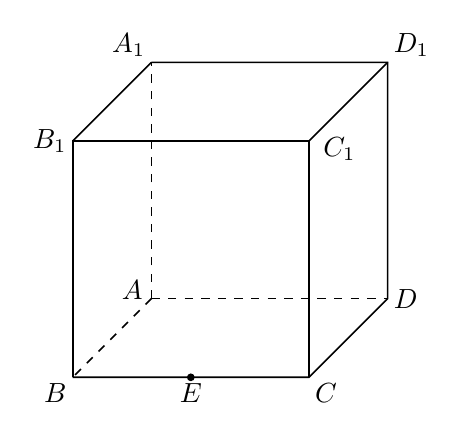
\begin{tikzpicture}[x=1cm,y=1cm,font=\normalsize,
  solidedge/.style={solid,line width=.6pt,draw=black},
  hidedge/.style={dashed,line width=.6pt,draw=black},
  ptlabel/.style={font=\normalsize,inner sep=2pt}]
\coordinate (B) at (0,0);
\coordinate (C) at (3,0);
\coordinate (A) at (1,1);
\coordinate (D) at (4,1);
\coordinate (B1) at (0,3);
\coordinate (C1) at (3,3);
\coordinate (A1) at (1,4);
\coordinate (D1) at (4,4);
\coordinate (E) at (1.5,0);
% 可见轮廓
\draw[solidedge] (B) -- (C) -- (D) -- (D1) -- (A1);
\draw[solidedge] (B) -- (B1) -- (C1) -- (C);
\draw[solidedge] (B1) -- (A1);
\draw[solidedge] (C1) -- (D1);
\draw[solidedge] (D) -- (D1);
% 遮挡棱（交于 A）
\draw[hidedge] (A) -- (B);
\draw[hidedge] (A) -- (D);
\draw[hidedge] (A) -- (A1);
\fill (E) circle (1.4pt);
\node[ptlabel,below left] at (B) {$B$};
\node[ptlabel,below right] at (C) {$C$};
\node[ptlabel,below] at (E) {$E$};
\node[ptlabel,left,xshift=-1pt,yshift=3pt] at (A) {$A$};
\node[ptlabel,right] at (D) {$D$};
\node[ptlabel,left] at (B1) {$B_{1}$};
\node[ptlabel,right,xshift=3pt,yshift=-3pt] at (C1) {$C_{1}$};
\node[ptlabel,above left] at (A1) {$A_{1}$};
\node[ptlabel,above right] at (D1) {$D_{1}$};
\end{tikzpicture}
